\documentclass{standalone}
\usepackage{tikz}
\usetikzlibrary{patterns, positioning}
\usepackage[sfdefault]{ClearSans} %% option 'sfdefault' activates Clear Sans as the default text font
\usepackage[T1]{fontenc}

\begin{document}
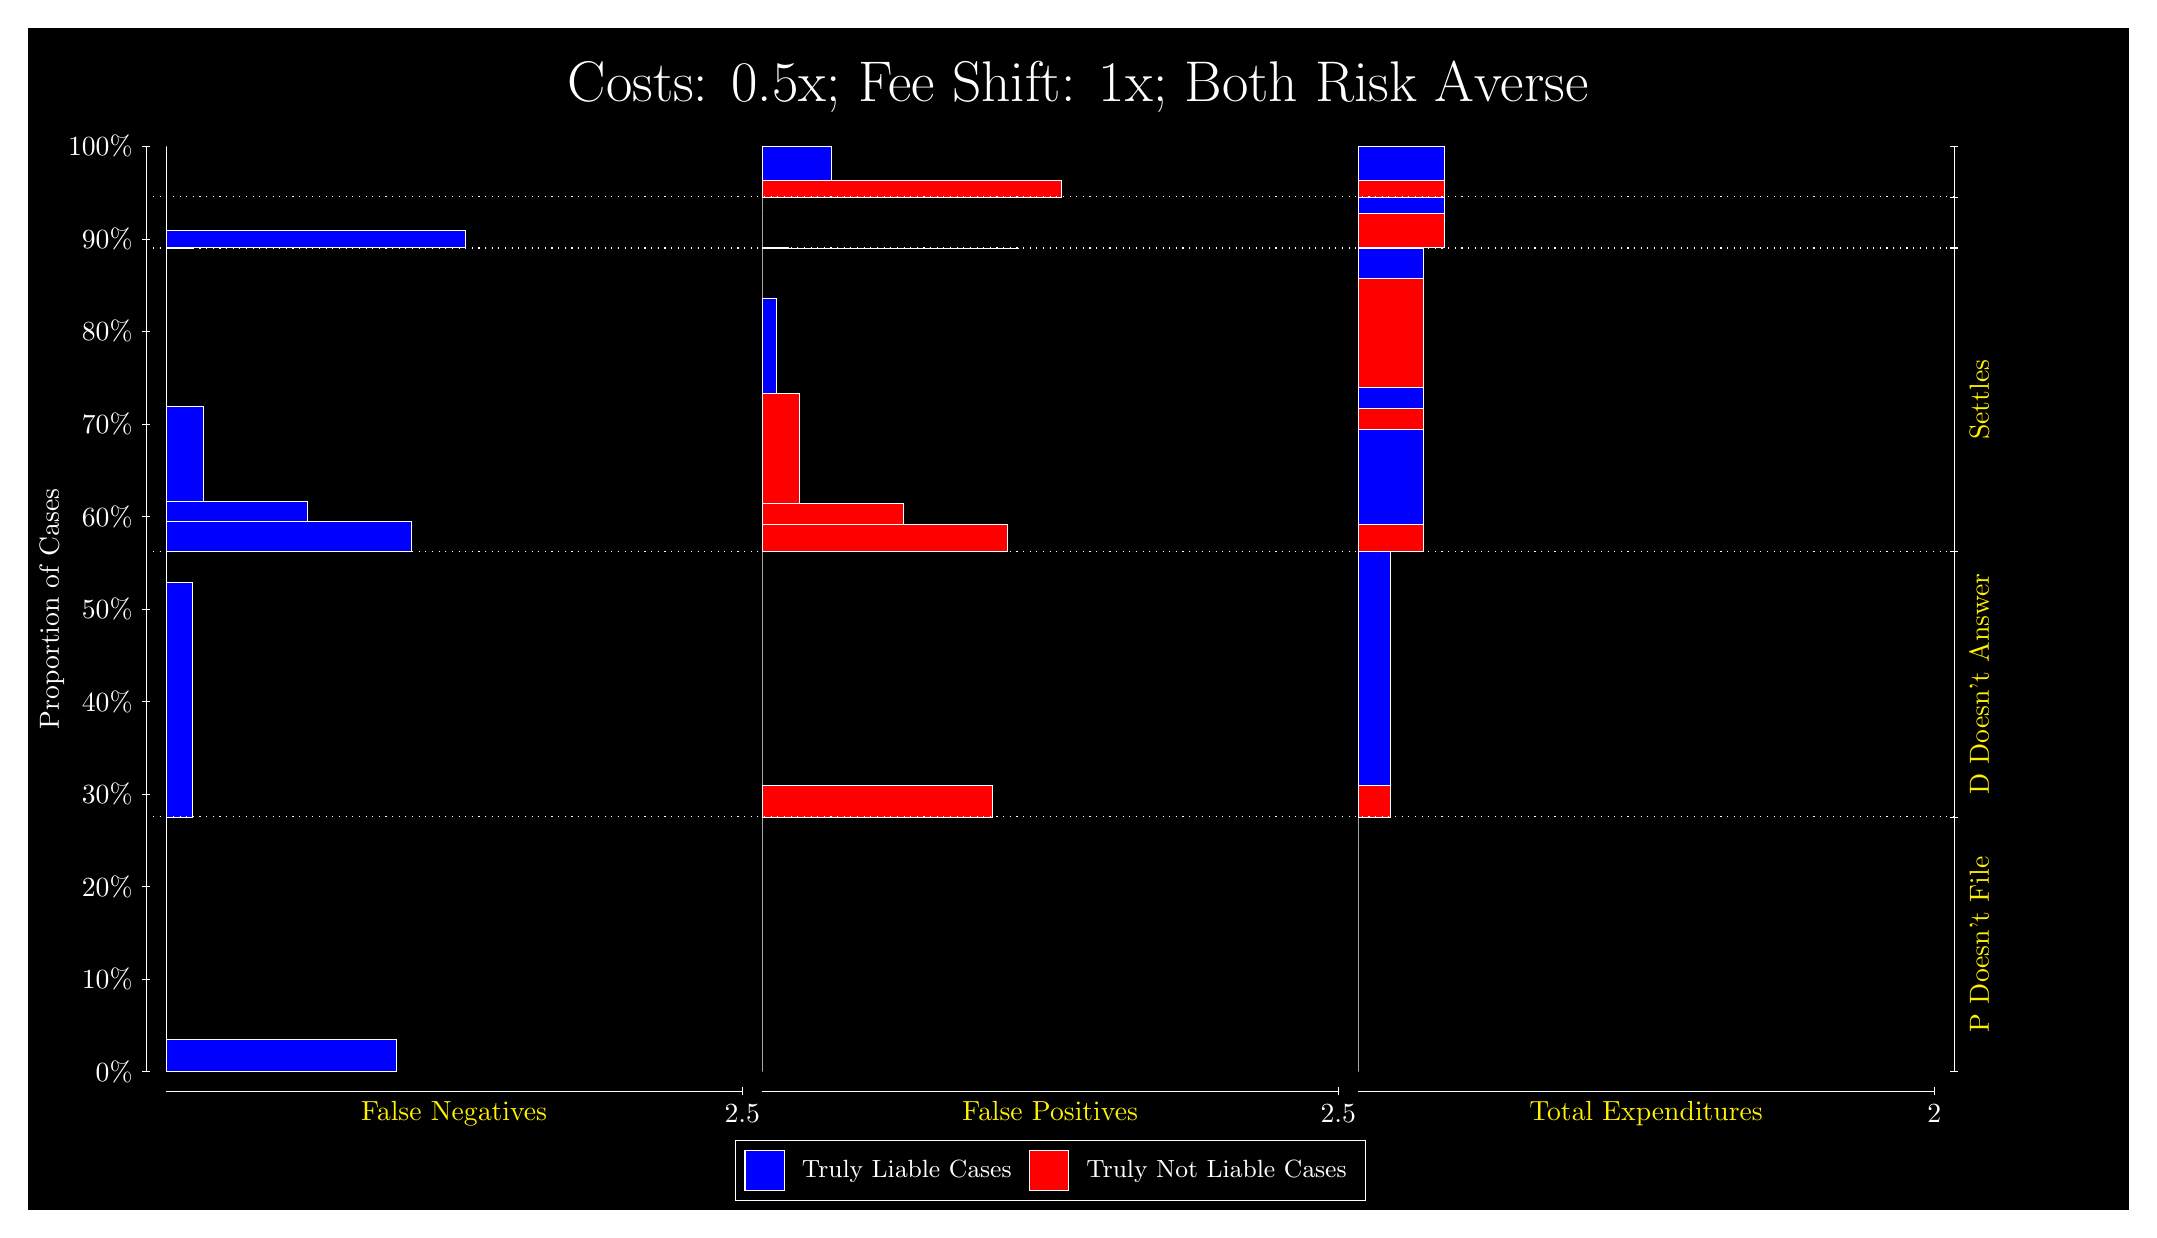
\begin{tikzpicture}
\draw[fill=black] (0,0) rectangle (26.667,15);
\draw[text=white] (0,13.5) rectangle (26.667,15) node[midway] {\huge Costs: 0.5x; Fee Shift: 1x; Both Risk Averse};
\draw[white, very thin] (1.5,1.75) -- (1.5,13.5);
\node[rotate=90, text=white, anchor=center] at (0.3, 7.625) {Proportion of Cases};
\draw[white, very thin] (1.45,1.75) -- (1.55,1.75);
\node[text=white, anchor=east] at (1.45, 1.75) {0\%};
\draw[white, very thin] (1.45,2.925) -- (1.55,2.925);
\node[text=white, anchor=east] at (1.45, 2.925) {10\%};
\draw[white, very thin] (1.45,4.1) -- (1.55,4.1);
\node[text=white, anchor=east] at (1.45, 4.1) {20\%};
\draw[white, very thin] (1.45,5.275) -- (1.55,5.275);
\node[text=white, anchor=east] at (1.45, 5.275) {30\%};
\draw[white, very thin] (1.45,6.45) -- (1.55,6.45);
\node[text=white, anchor=east] at (1.45, 6.45) {40\%};
\draw[white, very thin] (1.45,7.625) -- (1.55,7.625);
\node[text=white, anchor=east] at (1.45, 7.625) {50\%};
\draw[white, very thin] (1.45,8.8) -- (1.55,8.8);
\node[text=white, anchor=east] at (1.45, 8.8) {60\%};
\draw[white, very thin] (1.45,9.975) -- (1.55,9.975);
\node[text=white, anchor=east] at (1.45, 9.975) {70\%};
\draw[white, very thin] (1.45,11.15) -- (1.55,11.15);
\node[text=white, anchor=east] at (1.45, 11.15) {80\%};
\draw[white, very thin] (1.45,12.325) -- (1.55,12.325);
\node[text=white, anchor=east] at (1.45, 12.325) {90\%};
\draw[white, very thin] (1.45,13.5) -- (1.55,13.5);
\node[text=white, anchor=east] at (1.45, 13.5) {100\%};

\draw[white, very thin] (24.457,1.75) -- (24.457,13.5);
\draw[white, very thin] (24.407,1.75) -- (24.507,1.75);
\node[anchor=west] at (24.407, 1.75) {};
\draw[white, very thin] (24.407,4.9834) -- (24.507,4.9834);
\node[anchor=west] at (24.407, 4.9834) {};
\draw[white, very thin] (24.407,8.3573) -- (24.507,8.3573);
\node[anchor=west] at (24.407, 8.3573) {};
\draw[white, very thin] (24.407,12.204) -- (24.507,12.204);
\node[anchor=west] at (24.407, 12.204) {};
\draw[white, very thin] (24.407,12.219) -- (24.507,12.219);
\node[anchor=west] at (24.407, 12.219) {};
\draw[white, very thin] (24.407,12.859) -- (24.507,12.859);
\node[anchor=west] at (24.407, 12.859) {};
\draw[white, very thin] (24.407,13.5) -- (24.507,13.5);
\node[anchor=west] at (24.407, 13.5) {};

\draw[white, very thin, fill=blue] (1.75,1.75) rectangle (4.6775,2.1547);
\draw[white, very thin, fill=red] (1.75,2.1547) rectangle (1.75,4.9834);
\draw[white, very thin, fill=blue] (1.75,4.9834) rectangle (2.0793,7.9579);
\draw[white, very thin, fill=red] (1.75,7.9579) rectangle (1.75,8.3573);
\draw[white, very thin, fill=blue] (1.75,8.3573) rectangle (4.8605,8.7323);
\draw[white, very thin, fill=blue] (1.75,8.7323) rectangle (3.5431,8.9909);
\draw[white, very thin, fill=blue] (1.75,8.9909) rectangle (2.2257,10.202);
\draw[white, very thin, fill=red] (1.75,10.202) rectangle (1.75,12.204);
\draw[white, very thin, fill=blue] (1.75,12.204) rectangle (2.0793,12.215);
\draw[white, very thin, fill=red] (1.75,12.215) rectangle (1.75,12.219);
\draw[white, very thin, fill=blue] (1.75,12.219) rectangle (5.5558,12.433);
\draw[white, very thin, fill=red] (1.75,12.433) rectangle (1.75,12.859);
\draw[white, very thin, fill=red] (1.75,12.859) rectangle (1.75,13.074);
\draw[white, very thin, fill=blue] (1.75,13.074) rectangle (1.75,13.5);
\draw[white, very thin, fill=red] (9.3189,1.75) rectangle (9.3189,4.5787);
\draw[white, very thin, fill=blue] (9.3189,4.5787) rectangle (9.3189,4.9834);
\draw[white, very thin, fill=red] (9.3189,4.9834) rectangle (12.246,5.3829);
\draw[white, very thin, fill=blue] (9.3189,5.3829) rectangle (9.3189,8.3573);
\draw[white, very thin, fill=red] (9.3189,8.3573) rectangle (12.429,8.7007);
\draw[white, very thin, fill=red] (9.3189,8.7007) rectangle (11.112,8.9681);
\draw[white, very thin, fill=red] (9.3189,8.9681) rectangle (9.7946,10.36);
\draw[white, very thin, fill=blue] (9.3189,10.36) rectangle (9.5018,11.571);
\draw[white, very thin, fill=blue] (9.3189,11.571) rectangle (9.3189,12.204);
\draw[white, very thin, fill=red] (9.3189,12.204) rectangle (12.576,12.208);
\draw[white, very thin, fill=blue] (9.3189,12.208) rectangle (9.6482,12.219);
\draw[white, very thin, fill=red] (9.3189,12.219) rectangle (9.3189,12.644);
\draw[white, very thin, fill=blue] (9.3189,12.644) rectangle (9.3189,12.859);
\draw[white, very thin, fill=red] (9.3189,12.859) rectangle (13.125,13.074);
\draw[white, very thin, fill=blue] (9.3189,13.074) rectangle (10.197,13.5);
\draw[white, very thin, fill=red] (16.888,1.75) rectangle (16.888,4.5787);
\draw[white, very thin, fill=blue] (16.888,4.5787) rectangle (16.888,4.9834);
\draw[white, very thin, fill=red] (16.888,4.9834) rectangle (17.299,5.3829);
\draw[white, very thin, fill=blue] (16.888,5.3829) rectangle (17.299,8.3573);
\draw[white, very thin, fill=red] (16.888,8.3573) rectangle (17.711,8.7007);
\draw[white, very thin, fill=blue] (16.888,8.7007) rectangle (17.711,9.9116);
\draw[white, very thin, fill=red] (16.888,9.9116) rectangle (17.711,10.179);
\draw[white, very thin, fill=blue] (16.888,10.179) rectangle (17.711,10.438);
\draw[white, very thin, fill=red] (16.888,10.438) rectangle (17.711,11.829);
\draw[white, very thin, fill=blue] (16.888,11.829) rectangle (17.711,12.204);
\draw[white, very thin, fill=red] (16.888,12.204) rectangle (17.711,12.208);
\draw[white, very thin, fill=blue] (16.888,12.208) rectangle (17.711,12.219);
\draw[white, very thin, fill=red] (16.888,12.219) rectangle (17.986,12.644);
\draw[white, very thin, fill=blue] (16.888,12.644) rectangle (17.986,12.859);
\draw[white, very thin, fill=red] (16.888,12.859) rectangle (17.986,13.074);
\draw[white, very thin, fill=blue] (16.888,13.074) rectangle (17.986,13.5);
\draw[white, dotted] (1.5,4.9834) -- (24.457,4.9834);
\draw[white, dotted] (1.5,8.3573) -- (24.457,8.3573);
\draw[white, dotted] (1.5,12.204) -- (24.457,12.204);
\draw[white, dotted] (1.5,12.219) -- (24.457,12.219);
\draw[white, dotted] (1.5,12.859) -- (24.457,12.859);
\draw[white, very thin] (1.75,1.5) -- (9.0689,1.5);
\node[text=yellow, anchor=north] at (5.4094, 1.5) {False Negatives};
\draw[white, very thin] (9.0689,1.45) -- (9.0689,1.55);
\node[text=white, anchor=north] at (9.0689, 1.45) {2.5};

\draw[white, very thin] (9.3189,1.5) -- (16.638,1.5);
\node[text=yellow, anchor=north] at (12.978, 1.5) {False Positives};
\draw[white, very thin] (16.638,1.45) -- (16.638,1.55);
\node[text=white, anchor=north] at (16.638, 1.45) {2.5};

\draw[white, very thin] (16.888,1.5) -- (24.207,1.5);
\node[text=yellow, anchor=north] at (20.547, 1.5) {Total Expenditures};
\draw[white, very thin] (24.207,1.45) -- (24.207,1.55);
\node[text=white, anchor=north] at (24.207, 1.45) {2};

\node[text=yellow, centered, rotate=90] at (24.777, 3.3667) {P Doesn't File};
\node[text=yellow, centered, rotate=90] at (24.777, 6.6704) {D Doesn't Answer};
\node[text=yellow, centered, rotate=90] at (24.777, 10.281) {Settles};




\draw (12.978300999999998,1.5) node[draw=none] (baseCoordinate) {};
\begin{scope}[align=center]
        \matrix[scale=0.5, draw=white, below=0.5cm of baseCoordinate, nodes={draw}, column sep=0.1cm]{
            \node[rectangle, draw, minimum width=0.5cm, minimum height=0.5cm, fill=blue] {}; &
            \node[draw=none, font=\small, text=white] (B) {Truly Liable Cases}; &
            \node[rectangle, draw, minimum width=0.5cm, minimum height=0.5cm, fill=red] {}; &
            \node[draw=none, font=\small, text=white] (B) {Truly Not Liable Cases}; \\
            };
\end{scope}

\end{tikzpicture}
\end{document}